\documentclass[12pt]{article}

% Packages
\usepackage[hidelinks]{hyperref}
\usepackage{fancyhdr}
\usepackage{titlesec}
\usepackage{url}
\usepackage{graphicx}

\newcommand{\HRule}{\rule{\linewidth}{0.5mm}}

% Header and Footer
\pagestyle{fancy}
\fancyhf{}
\lhead{[Name of the app/project] Report}
\rhead{Programming 2 (CM12005)}
\cfoot{\thepage}
\setlength{\headheight}{14.5pt}

% Adjust the spacing of the section titles
\titleformat{\section}{\Large\bfseries}{\thesection}{1em}{}
\titlespacing{\section}{0pt}{*0.5}{*0.5}

\begin{document}

% Title Page
\begin{titlepage}
    \centering
    {\Huge \bfseries [Name of the App/Project]}\\[0.2cm]
    \vspace*{0.5cm}
    {\large Author 1, Author 2, Author 3, Author 4, Author 5, Author 6, Author 7, Author 8, Author 9}\\[2cm] % Authors
    \vspace*{1cm}

    \begin{minipage}{0.9\textwidth}

        \textbf{Abstract:} About 200 words here. Lorem ipsum aliquam
        etiam erat velit scelerisque in dictum non consectetur a erat nam at lectus
        urna duis convallis convallis tellus id interdum velit laoreet id donec
        ultrices tincidunt arcu non sodales neque sodales ut etiam sit amet nisl
        purus in mollis nunc sed id semper risus in hendrerit gravida rutrum
        quisque non tellus orci ac auctor augue mauris augue neque gravida in
        fermentum et sollicitudin ac orci phasellus egestas tellus rutrum tellus
        pellentesque eu tincidunt tortor aliquam nulla facilisi cras fermentum odio
        eu feugiat pretium nibh ipsum consequat nisl vel pretium lectus quam id leo
        in vitae turpis massa sed elementum tempus egestas sed sed risus pretium
        quam vulputate dignissim suspendisse in est ante in nibh mauris cursus
        mattis molestie a iaculis at erat pellentesque adipiscing commodo elit at
        imperdiet dui accumsan sit amet nulla facilisi morbi tempus iaculis urna id
        volutpat lacus laoreet non curabitur gravida arcu ac tortor dignissim
        convallis aenean et tortor at risus viverra adipiscing at in tellus integer
        feugiat scelerisque varius morbi enim nunc faucibus a pellentesque sit amet
        porttitor eget dolor morbi non arcu risus quis varius quam quisque id diam
        vel quam elementum pulvinar etiam non quam lacus suspendisse faucibus
        interdum posuere lorem.

    \end{minipage}
\end{titlepage}
\thispagestyle{fancy}

\newpage

\tableofcontents
\thispagestyle{empty}

\newpage

\setcounter{page}{1}

\section{Introduction (2 pages)}
Increasingly, medical advice and research is showing that minor changes to an individual’s daily routines can have positive effects on their overall health, wellbeing and productivity. For example, we are often reminded of the advantages of walking 10,000 steps (Tudor-Locke et al., 2011), sleeping for at least 7 hours (Watson et al., 2015) and drinking at least 6 cups of water (NHS, 2023) every day. However, as discussed by Madore and Wagner (2019), processing multiple tasks concurrently can lead to reduced efficiency. Therefore, tools to aid in the tracking and pursuing of these personal development goals are likely to help an individual reach their goals more effectively.\par

PI(Personal Informatics) software is software designed to help collect and analyse data about an individual with the aim of promoting self-understanding and betterment. A PI system could be an ideal solution to this issue as it could be very useful in allowing an individual to monitor and streamline their progress towards their goals for self-improvement.\par

However, in designing a PI system it is important to ensure user engagement; if a user stops using a system then the system cannot help them. Kersten-van Dijk et al. (2017) found that the studies they reviewed which discussed users dropping out of using a PI system reported dropout rates of 7-44\%. This suggests that a significant proportion of people might not feel motivated to continue using PI software. Furthermore, Jones and Kelly (2018) found that presenting users with too much information could leave them feeling overwhelmed; Rapp and Cena (2016) found that first-time users of PI systems could find the act of recording their data burdensome; and Potapov et al. (2021) discovered that teenagers often found PI systems either controlling or confusing depending on the way they were designed.\par

Fortunately, some of these studies, as well as many others, have investigated how to make a PI software system effective for its users and proposed ways of designing systems with this in mind. For instance, Jones and Kelly (2018) suggested that, to avoid overwhelming users, a system should only show the user information that is interesting to them. They found that 'interesting information' was that which was surprising, useful or statistically significant. It was also found that users found it more interesting when insights could be provided between aspects of their life, rather than within them. Rapp and Cena (2016) recommended providing users with tailored summaries and targets; control over their data; and reviews of past data. In this way they suggested that feelings of freedom and nostalgia might be fostered, increasing positive views and connections with the software. Potapov et al. emphasise the importance of finding an appropriate balance between constraints to orient the user towards positive goals and freedom to allow them to use the tool in a way that suits them. Additionally, a study by Loerakker et al. (2023) showed that promoting self-compassion through the design of a Personal Informatics system can foster positive self-reflection while reducing the chances of rumination and cessation of goal pursuit. The study showed that framing data positively can promote self-compassion. For example, highlighting positive achievements rather than criticising poorer performance.\par

Our intention is to create a PI system aimed at current university students. To  decide on a list of metrics for our system to track, we investigated the interests of our chosen demographic by means of a Google Forms survey. The survey, which was sent to students online, revealed that 60\% of respondents were most interested in tracking their health, followed by 30\% who were most interested in tracking their own learning and development. In addition, when asked to rate their interest in tracking their data for self-improvement on a scale of 1-10, 55\% of participants rated their interest at 8 or above. This reinforced our belief that a PI system would be popular among our target audience. We also conducted some individual interviews of students involving more specific questions about health and desirable PI system features. These interviews revealed an interest in graphs and a simple user interface which we will take into account when designing our application. All the students we interviewed also expressed a desire to alter the number of hours of sleep they got on a daily basis. Based on these investigations, as well as research into Fitbit and Garmin software, we decided that our system would track hours of sleep, water intake, steps taken and hours spent productively.\par

Our system will allow data to be entered manually. Some metrics will also be able to collect data automatically via the Fitbit API to reduce the burden of data entry. Additionally, our software will allow users to set personal goals and see useful data about their performance. This data will be able to showcase correlation in each metric against time individually and between separate metrics. This functionality will all be accessed via a desktop application with a graphical user interface. We hope that, by tracking these four important aspects of student life, our system will provide interesting and useful insights that guide our users towards better health and productivity while ensuring that they are not overwhelmed by too much data or the need to balance their goals.


\section{Agile Software Process Planning and Management (2 pages)}
\textbf{This section must describe how you carried out your project as an Agile process, including
how you planned and tracked your sprints, and how Scrum meetings were used to manage
the evolution of your idea and the features you decided to include in your software system.}\par
To carry out this project in an efficient and organised manner, we followed Agile practices and values using the Scrum framework. This involved using a series of week-long sprints to break up and work through the continuously evolving product backlog. Between each sprint, a meeting was held to discuss the outcome of the previous sprint, go over any changes to the product backlog, produce a sprint backlog and divide this sprint backlog between the group members for completion during the next sprint. To maintain clarity and access to information, minutes were taken of these meetings and stored in the project GitHub repository. This meant that developers could always access information about the progress of other developers and their allocated tasks (See Appendix x). During sprints, group members worked either individually or as part of a smaller group to complete their allocated element of the sprint backlog. Regular scrum meetings were also used to allow group members to communicate progress, plans, obstacles and key information. We assigned a scrum master to gain a full understanding of Agile values and methodologies and ensure the group's adherence to them. A product owner was also chosen to be in charge of managing the product backlog and organising sprints.\par

Our first sprint was devoted towards research into PI systems and what students wanted in one. Three group members were assigned to researching PI systems, two to market research, two to gauging interest in students, one to compiling the initial project backlog and one to researching the most appropriate programming language to use for the project. By the end of the week, all members had fulfilled the duties assigned to them. The research was discussed as a group and used to produce the idea for our system. As this idea evolved, it was converted into a list of functional requirements and added to the product backlog.\par

The second sprint consisted of designing and beginning to create our application. A member of the team set up a framework for our project on GitHub and two team members were assigned the task of creating a UI (User Interface) diagram for our application. Having done this, the UI designers presented the result in a scrum meeting and, based on this, other members of the group created a coding plan, started creating the UI and implemented some basic functionality. Meanwhile, a group member worked on creating a database and demonstrating the use of it; another researched and showcased the use of a suitable API; and the remaining people began the writing of the report. The scrum meetings held throughout the week were key in ensuring that all the programmers could stay abreast of any important changes made by others with impacts on their own work, as well as allowing the sharing and discussion of issues. At the end of the sprint, all available team members attended a Google Meet meeting in which all progress was discussed. The sprint was very successful, with every individual achieving their designated goals. Based on the API research conducted, it was decided that the Fitbit API was most suitable for our system. Additionally, it was concluded that an alternative database design would be more efficient. These evolutions of the idea of our project meant that the product backlog was updated.\par

The sprint that followed largely prioritised the implementation of desired functionalities from the product backlog. Five members of the group were individually allocated to specific aspects of the program. This included implementing the productivity tracker, achievements, goals, graphs and the Fitbit API integration. One developer was also assigned to redesigning the database to be more efficient. The other available group members were given sections of the report to work on. During the frequent scrum meetings in this sprint, reporting back helped maintain a full understanding of the latest changes among the programmers. Unfortunately, due to technical difficulties, the sprint backlog was not entirely completed. These incomplete tasks were added to the sprint backlog of the next sprint. Other than some software features, all tasks were completed successfully and the next sprint was discussed and planned as usual.\par

The fourth sprint had very similar aims to the previous one, with team members allocated to report writing and the development of features, including those which were not completed during the previous week. By the end of the sprint, more elements of our system's functionality had been implemented and the report completed further so these parts of the product backlog were marked as complete. However, the design section of the report and the achievement functionality of the system were not completed due to other commitments and the work tracking section was not fully functional due to technical difficulties. The completion of these requirements was moved to the following week's sprint.\par

The fifth, and final, sprint targeted the completion of as yet unimplemented features and work on the report document. These responsibilities were split so that roughly half the group was working on each. As well as the programming of parts of the system, focus was also placed on merging all the functionality together to create our system as a whole.


\newpage
\section{Specification of Software Requirements}

This section establishes the core requirements for our Personal Informatics
(PI) system, focusing on helping students keep up with their fitness and study
goals. We utilised feedback from surveys, talks with users, market research,
and academic research articles to figure out what features our system should have. Our
aim is to make a system that assists students in improving both their physical
health and studying habits whilst not being overly invasive.


\subsection{Gathering System Requirements}

Initially, we asked people what features they would look for in an personal
improvement application. From these interviews, we identified that most students use PI systems for
tracking their fitness (60\%) and their learning progress (30\%), with the other 10\% being interested in their environmental impact. This
helped us decide which area of personal informatics our system should focus on. Next, we looked
at what users stated about our initial ideas as well as comparing our ideas
to expert findings from our listed articles. Additionally, many students told us they prefer applications
that are intuitive but still allow for great insight and control into goals
and targets. Also, they wished to connect with their friends and peers through the app and
liked the idea of seeing all their information in a single area. Furthermore, we also researched into competitor 
systems (such as garmin and fitbit) to identify both good and bad features of these systems.\par

After this, we made a final list of what functionality our app must contain based on the data gathered. We must
ensure our system is perfect for tracking health and study time, allows users
to share their progress with friends, and keeps all their data safe and
private.
 

\subsection{Specific Domain of Application}

Our PI system is intricately designed with a student demographic at its core,
addressing their unique challenges such as managing academic deadlines
alongside maintaining a balanced lifestyle.\par 

Students grapple with the dual challenges of academic accountability and
physical well-being. The system shall provide a suite of tools for effective
study habits and simple health tracking.
 

\subsection{Data Fields Chosen}

Our app is tailored towards individuals who require assistance managing their time healthily as
we are aware that a large proportion of students have difficulty maintaining a healthy work-life
balace. Our app aims to help them track key aspects of the student lifestyle.
The fields we have chosen to track are as follows:

\begin{itemize}

    \item \textbf{Tracking sleep time}: The average student struggles to manage sleep, studying, and being social and out of these three, sleep is usually the area in which students choose to disregard in order to create more time. However, a lack of sleep can be detrimental on all aspects of life and as such it is imperative that we ensure our users are aware of how little sleep thay may be getting across a given time frame. We are aware that some students may also be getting too much sleep which can lead to them feeling lethargic throughout the day and as such our system should also provide a solution for these users. Sleep quality also plays a large role in this but is incredibly difficult to track unless specialist equipment is used. Additionally, it is usually influenced by factors our system cannot control such as noise from other tenants and temperature.

This field will require a user to manually enter their data **or tracked by a fitbit, depends on the coding**. Allowing a user to set goals for this field will enable them to prioritise the quantity of sleep they are getting each night. Our system should enable our users to obtain a consistent, healthy sleep pattern
    
    \item \textbf{Tracking step count}: The average student spends a large proportion of their day sedentry, whether that be from napping after a lecture, studying hard for an exam, or sat behind a computer trying to finish coursework. This can cause students to not get out frequently for events other than their lectures and the occasional social gathering. This has hidden consequences: less time outside walking means less vitamin D, less opportunity to make new friends, increased risk of certain diseases such as heart disease. It is imperative to emphasise to our users who do not perform enough steps in a given time period that this behaviour is not healthy. Our system will allow a user to view trends in their step data and clearly visualise how litte (or many) steps they are actually performing.

    \item \textbf{Tracking work done}: Students often report one of two extremes when it comes to studying: overstudying and losing out on other aspects of the student life or understudying and suffering academically. Neither of these are healthy for a student. To potentially fix this behaviour, our system should allow a user to set study goals. This allows the understudying students to have a target to achieve in a given time period, motivating them to allocate more time to study. Furthermore, this allows the overstudying students to know that they have studied a sufficient amount for a given time period and deserve a break.
    
    \item \textbf{Tracking water intake}: Water intake has many hidden benefits: helps with weight loss by making you feel more full, increases energy levels, improves skin health. Many students may neglect drinking water as they need an energy boosted via caffeinated products. By setting clear goals of how much water a user should drink, it increases the likelihood they select to drink water over a less healthy alternative.

    \item \textbf{Achievements}: This will be the method by which goals for a user to achieve are set. Their main purpose is to motivate a user to change some aspect of their life. Through our research, we discovered that by providing some sort of challenge, a user becomes more motivated to complete a goal, even if no physical reward (aside from health benefits) is provided. By allowing the user to set these goals we ensure that the user finds these achievements to be possible and further increases the likelihood they change some of their bad habits.

\end{itemize}


\subsection{Allow Users to Manage Goals}

Our system will allow users to set and manage goals via an achievement system. These achievements can be manually set or removed by the user. We are using achievements as they provide a reason for a user to improve specific fields without aimlessly trying to increase some number. Furthermore, these achievements can take place over different ranges of time: day, week to date, month to date, year to date.


\subsection{Comparing User Data}

Our system must ensure that a user can compare all data fields in an intuitive manner. This will be done via graphs that allow the user to select what fields they wish to view along with a time frame (day, week, month to date, year to date).
By including time frames, the user can identify potential outside factor that our system cannot consider. For example, an event in a given time frame such as a coursework deadline could influence sleep count. The user could then use this data to come up with ways to improve their behaviour patterns for other similar circumstances in the future.


\subsection{Viewing and Collecting Tracking Data}
A large portion of any given user's data (provided they own a fitbit device or have used the fitbit app) is going to be accessed via the fitbit API upon request from each user. We must ensure that potential users without the relevant hardware can still use our system and must be done in an intuitive way in order to allow our system to be accessible for a greater amount of students. This will also allow for easy gathering of data fields which cannot be tracked via physical devices. As not all data fields we have selected can be accessed directly via the fitbit API (sleep, and study time), manual entry is necessary.\newline

To ensure that our users understand what data we are storing, each user shall be allowed to view the data we have stored on them for each of these key fields.
In addition, the security of this data is paramount. We must ensure it cannot be accessed by any other end users.


\subsection{Scalability and Performance}

Scalability will not be a problem for our system as it runs entirely off of the user's computer.\\

We must ensure that this system performs smoothly and efficiently to not hinder a user's experience.


\subsection{Structuring the Software Development Process}

Our development of this project very closely followed the agile and SCRUM development approach. This was done to ensure our system was consistently improving and changing to match what our users will need. This was done through weekly review meetings where our group would assemble and discuss if the goals for the sprint had been completed, ways to expand upon the work produced in each sprint, any potential issues with the goals set for the sprint. This was led by our scrum master who ensured that all goals for the week were thoroughly discussed and examined, along with taking minutes for each meeting to ensure that all members knew exactly what needed to be completed. Our sprints tended to last 1 week each, with goals consistently being met by the vast majority of the group. During each sprint, the group members focusing on developing the software would regularly discuss and assist each other via online meetings.\\


\subsection{Testing}
dunno what we're testing so this is empty :)

\newpage
\section{Design (5 pages)}
\subsection{Design description}
In the design of our Personal Informatics system, the UML diagrams serve as a cornerstone for understanding the structure and relationships within the application. The diagrams are organized to reflect the logical architecture of the system and consists of several key classes that correlate directly with the user data management and activity tracking functionalities.\par

The Entity-Relationship Diagram (ERD) illustrates the intricate structure of our Personal Informatics system, designed specifically for tracking and managing various user-centric activities. This diagram provides a visual representation of the data relationships and is critical in guiding the development process to ensure the system meets both functional and non-functional requirements effectively.\par

\begin{figure}[h!]
  \centering
  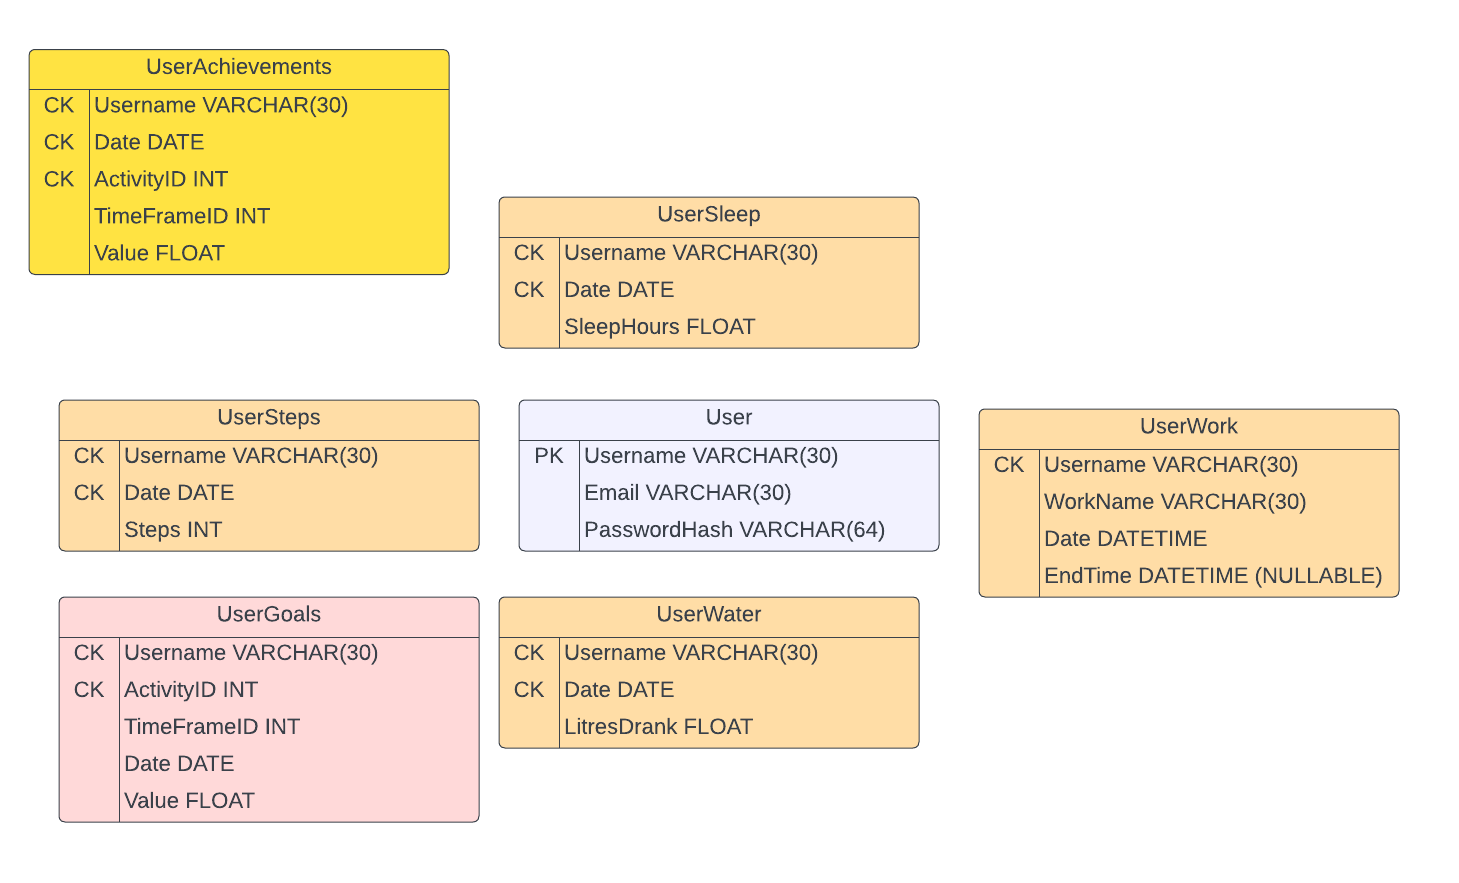
\includegraphics[width = \linewidth]{PI ERD}
  \caption{Database ERD model of our PI system}
  \label{fig:PI_ERD}
\end{figure}

User Class: Central to our system, the User class captures essential personal identifiers and account information for each user. Attributes include Username, Email, and Password, which are fundamental for ensuring secure user authentication and system access. This class acts as the primary entity with which other classes associate, establishing a one-to-many relationship across various data-tracking entities. Each instance of a User can associate with multiple records in subordinate classes, reflecting the diverse activities and metrics tracked by the system. However, at the end, we did not manage to implement the multi-user system, this can be a huge improvement if we have more time to build to application.\par

UserAchievements Class: This class stores specific achievements of users, linked directly to the User class. Attributes like Username, Date, ActivityID, TimeFrameID, and Value allow for detailed recording and analysis of user accomplishments across different activities and timeframes. It enables the system to provide feedback and insights based on historical achievement data, supporting motivational features such as goal setting and progress tracking.\par

UserStep Class: Dedicated to tracking the physical activity of steps taken, this class includes attributes such as Username, Date, and Steps. By recording daily step counts, the UserStep class feeds into the system’s health monitoring and fitness tracking capabilities, allowing users to set and monitor physical activity goals.\par

UserSleep Class: Focusing on sleep habits, this class records the duration of sleep per day for each user with attributes Username, Date, and SleepHour. It is vital for analyzing sleep patterns and correlating them with other health metrics, which is essential for offering personalized health insights and improving user well-being.\par

UserWork Class: This class tracks work and study sessions, an essential feature for our student users. Attributes include Username, WorkName, Date, and Endtime, facilitating the tracking of academic and work-related activities over time. This functionality supports students in managing their time and productivity more effectively.\par

UserWater Class: Monitoring hydration, the UserWater class includes attributes such as Username, Date, and LitresDrank. Hydration tracking is crucial for overall health, and this class allows the system to remind users to stay hydrated and track their daily water intake.\par

UserGoals Class: As a strategic component of our system, the UserGoals class holds data related to the personal objectives of users. With attributes like Username, ActivityID, TimeFrameID, Date, and Value, this class supports the setting and monitoring of personalized goals, enhancing the system's capability to drive user engagement and encourage behavior modification.\par

The class diagram of our Personal Informatics system delineates the fundamental components and their relationships, underscoring the system's design to efficiently manage and process user data. Central to this architecture is the Database class, which acts as the primary conduit for all data manipulation and retrieval activities within the system. This class is critical for the robust handling of data and supports various functionalities critical to user interaction and data integrity.\par

\begin{figure}[h!]
  \centering
  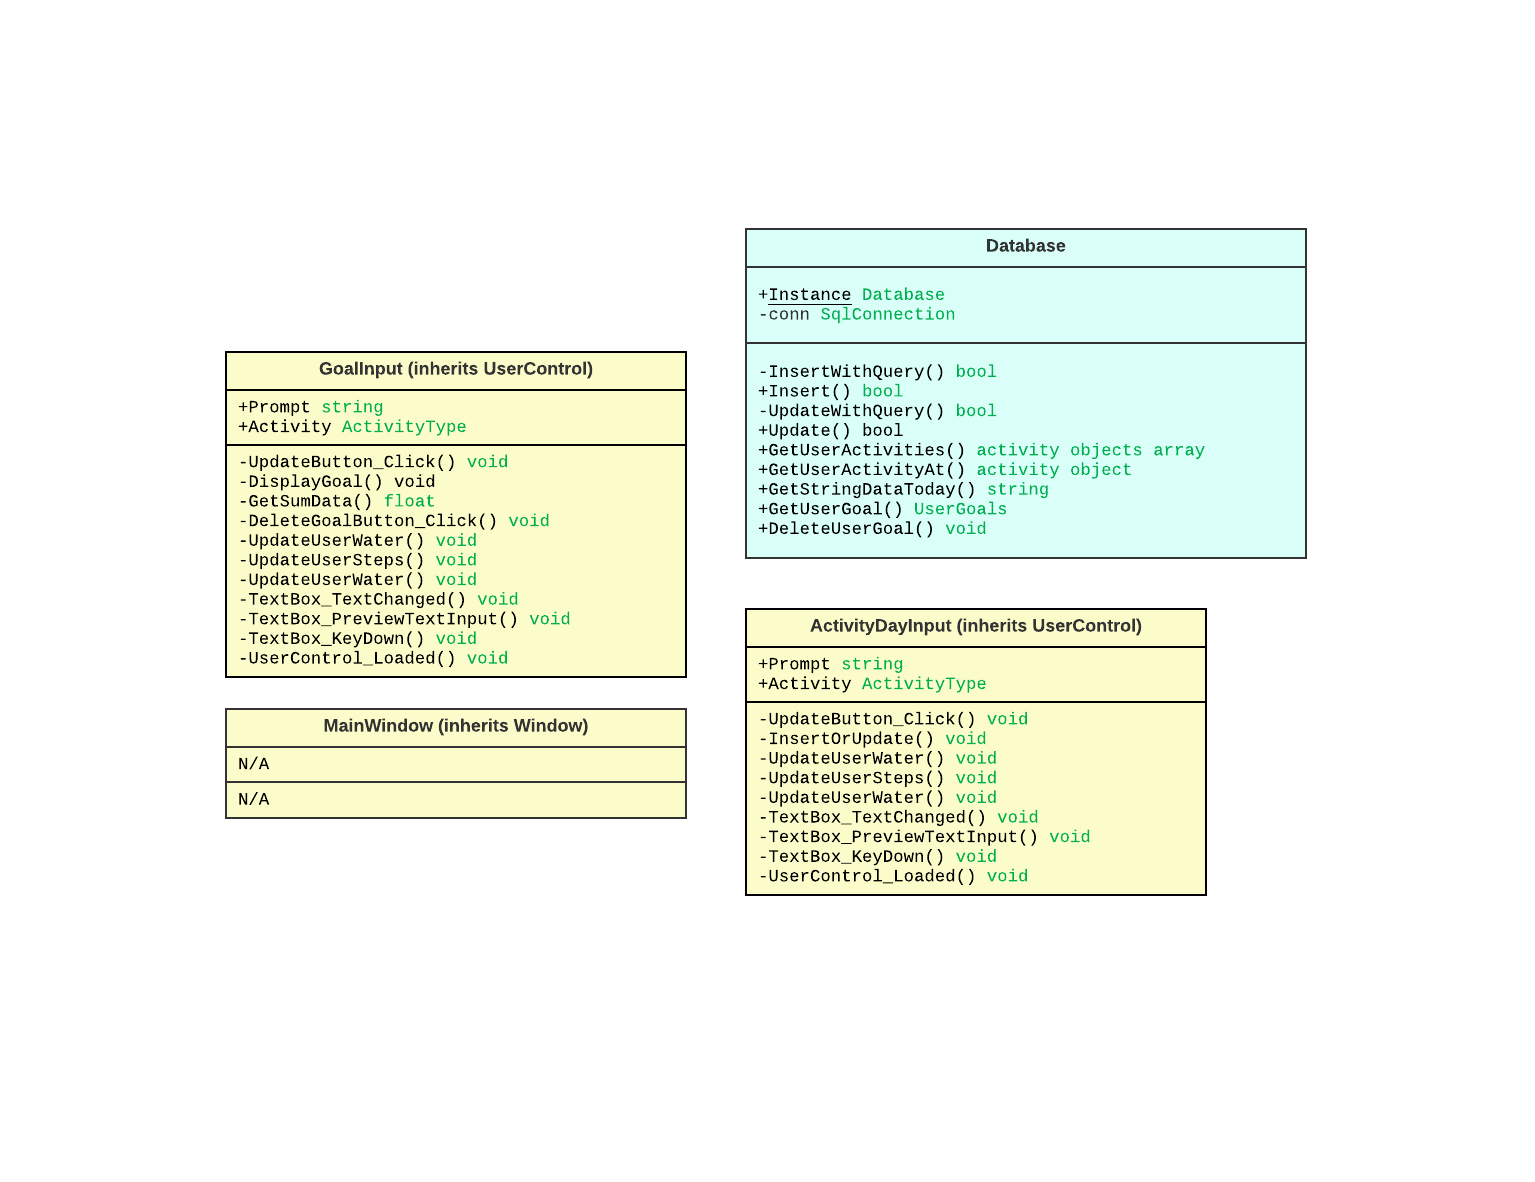
\includegraphics[width = \linewidth]{UML Class diagram}
  \caption{UML Class diagram of our PI system}
  \label{fig:Class}
\end{figure}

The Database class ensures a singleton pattern for database management, creating a single, globally accessible instance throughout the application lifecycle. It manages the database connectivity, facilitating secure and persistent connections to the data store. Data manipulation methods such as InsertWithQuery(), Insert(), UpdateWithQuery(), and Update() allow for efficient data insertion and updating within the database. Retrieval methods like GetUserActivities() and GetUserActivityAt() fetch activity data for users, crucial for generating reports and insights. Utility methods including GetStringDataToday(), GetUserGoal(), and DeleteUserGoal() provide additional functionality for managing daily data strings and user goals, enhancing the system’s responsiveness to user interactions.\par

The ActivityDayInput and GoalInput classes, both inheriting from UserControl, are specifically designed for handling the input and update functionalities related to daily user activities and goal management, respectively. The ActivityDayInput Class includes a Prompt string for user guidance and an Activity ActivityType to specify the type of activity data being entered. It comprises various user interaction handlers such as UpdateButton_Click() and InsertOrUpdate() for data submission, alongside UpdateUserWater() and UpdateUserSteps() for updating specific activity metrics. Text handling methods like TextBox_TextChanged(), TextBox_PreviewTextInput(), and TextBox_KeyDown() ensure data integrity and user input validation.\par

The GoalInput Class mirrors the ActivityDayInput class in providing prompts and activity type specifications tailored towards user goals. It features goal-specific functionalities such as DisplayGoal() for visualizing set goals, GetSumData() for data aggregation, and DeleteGoalButton_Click() for goal modification. It inherits text handling and initialization methods from ActivityDayInput, ensuring a consistent and user-friendly interface.\par

\begin{figure}[h!]
  \centering
  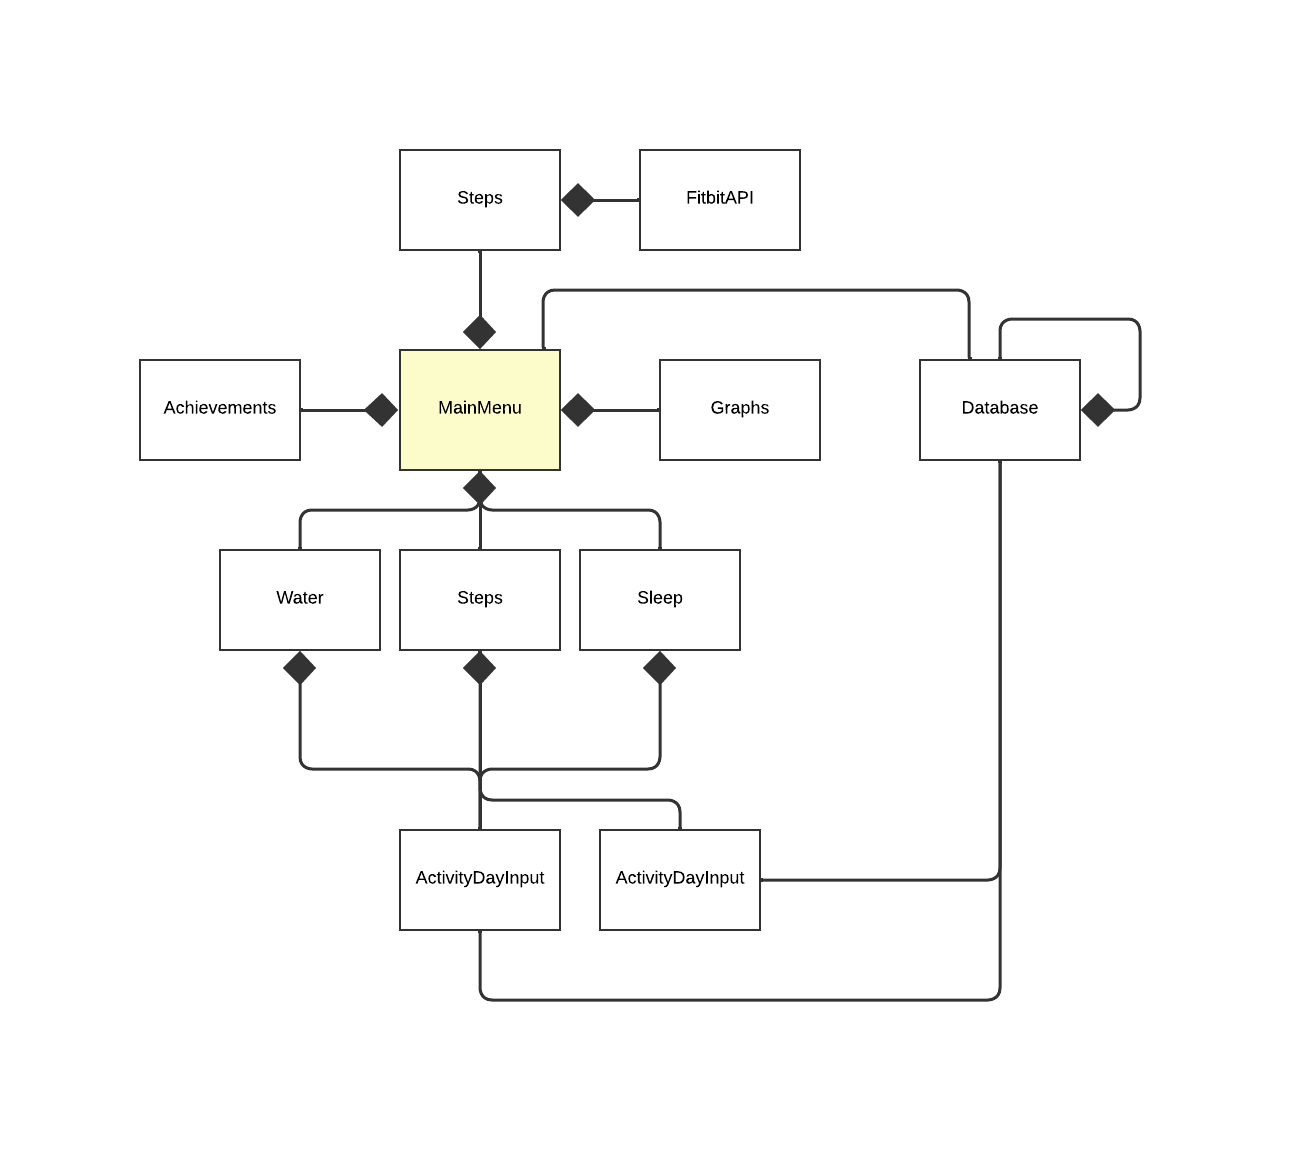
\includegraphics[width = \linewidth]{UML Flow diagram}
  \caption{UML Flow diagram of our PI system}
  \label{fig:flow}
\end{figure} 

The flow diagram of our Personal Informatics system illustrates the interactions between classes, essential for efficient functionality and user experience. At the core is the MainMenu class, which integrates features like tracking steps, achievements, water intake, and sleep via separate classes (Step, Achievement, Water, Sleep). These classes manage specific activities and are tightly integrated with ActivityDayInput and GoalInput controls for data entry and goal management.\par

For example, when users input their daily water intake through the ActivityDayInput tailored for water, this control processes and validates the data, then interacts with the Water class and the Database to store this information. Similarly, the GoalInput facilitates setting and updating goals, interacting directly with the Database to ensure goals are current and reflective of user activity.\par

The association between the ActivityDayInput, GoalInput, and the Database ensures immediate data reflection in the system, supporting features like activity comparison and trend analysis. The Database manages its instance, maintaining data integrity and security, and acts as a centralized repository for all user data. This structure ensures seamless data flow across the system, fulfilling functional and non-functional requirements, and enhancing overall user interaction.\par

\subsection{Design justification}
Functional requirement justification(Alex)

#*********** Begin *********
\textbf{Non-Functional Requierments:}

Like scpecified in A stage-based model of personal informatics systems (Li, Ian ; Dey, Anind ; Forlizzi, Jodi.  2010),  there are many factors that a PI system should be tailored towards to assure a constant interaction between the system and its users.  Our design was vagely tailores towards the 5 stages mentioned in A stage-based model of personal informatics systems (Li, Ian ; Dey, Anind ; Forlizzi, Jodi.  2010), these being Preparation Stage,  Collection Stage, Integration Stage,  Reflection Stage and Action Stage.  We made sure that users could chose what informatics they would prefer to track as well as how to record it, as we allowed API collection to be enabled or data to be manually inserted.\\

We generally offered useful but easy to gather data so that barriers such as difficulty in colletion would not interfere with our purpous,  and enabled users to compara their data between itself,  to watch for corelation.  For example,  a user could compare steps taken to sleep to see if having a proper walk directly correlates to sleep paterns,  and the user could even compare the data from last month, or in blocks of weeks to have a more aqurate messure.  These characteristics where tailored towards the Integration and Reflection Stage.  \\

Similarly,  the achievements page is aimed towards causing an action or a refelction in the user.  Our PI system allows users to set realistic goals for the day,  week or even month,  and rewards them with badges and motivating messages when these goals are met. Furthermore,  a streak counter increases every day that you achieve your goals,  and is reset if you fail to meet them.  This allows users to have a more competitive spirit towards themselves and maybe even thir friends.\\

From our multiple interviews, we gathered that people would respond positively to friendly competitions,  so we attempted to make a fun and interactive acheivements page that could be used to compare data and progress with other people.  To further expand upon this,  we made our data comparable with each other throiugh line graphs to effectivly see your progress throughout the day,  week or month,  and to further visualize your goals. \\

As we are perfectly aware that most people mut far more importance into one or two data types than the rest, we made it so that you can compare data with as many other types of data as you wish,  yet you could also concentrate on a specific one. \\

We wished for our PI system to be completely private if need be,  as even though we want friendly competitiveness between people,  the data being gathered could be quite sensitive,  and thorugh our interviews we gathered that making profiles private would be what most people would prefer.  Furthermore,  through these same interviews we found out that people would like to have goals and recomendations set by the PI,  as a sort of guide line for their objectives.  To implement this feature,  we devised the achievements page to provide our users with a ready made set of goals they should progressively aim towards.\\
#************* END ************
...\\

Non-functional\\
This design framework effectively meets the functional requirements such as data tracking, social features, and notifications by ensuring that each class is optimized for specific roles within the system. Non-functional requirements like usability, scalability, security, and performance are also adeptly addressed through this architecture. The system’s modular design allows for easy scalability and enhancements, while robust data handling ensures security and high performance, ensuring a responsive and reliable user experience. This meticulous organization not only supports operational efficiency but also enhances user engagement, thereby aligning with the overarching goal of the Personal Informatics system.\par

\section{Software Testing (Verification) (2 pages)}

This section should include:

Testing plans, indicating how you planned to perform verification of your PI system.
These plans should reflect your requirements and design work, and be completed
before any implementation (coding) work begins.

Evidence of testing - test case results.

During the initial planning of this project, the approach to testing was discussed. It was agreed that each time a developer completed a feature from the product backlog they would thoroughly white-box test it themselves using a variety of specifically chosen test cases and take screenshots to record the results. If all tests produced the desired results, the developer would consider the feature complete. If any tests were unsuccessful, however, they would debug and fix the problem before applying all tests again. In this way, the component's functionality given both valid and invalid inputs would be ensured. By testing each element before combining it with other elements of the system, the testing process as a whole would comprise a bottom-up integration testing approach. On the completion of a part of the product backlog, the developer would send the screenshots produced in testing to the product owner. The product owner would then analyse the screenshots to ensure that the evidenced functionality aligned with the requirements of the product backlog. The product owner would also use the screenshots to provide feedback to the developers and to inform future decisions and alterations to the product backlog.\par
\subsection{Example}
Below is the outcome of the testing of the --------- feature:

\section{Reflection and Conclusion (4 pages)}

This section should include two main sections:

A critique of your software system’s requirements specification, design and testing,
including what might be improved and why you feel it would be better with these
changes.

A critical reflection on the group’s software process, including evidence of Agility in
your software process, evidence of having evolved your requirements to reflect
changes in understanding of problem and viability of designs.


\section{References}

\renewcommand{\refname}{} 
\vspace{-20pt}
\begin{thebibliography}{99}
    % EXAMPLE 1
    \bibitem{ref-ex1} Surname, X. \textit{Article name} [Online].
    Available from:~\url{https://google.com}.

    % EXAMPLE 2
    \bibitem{ref-ex2} AfterAcademy, 2020. \textit{Sudoku Solver} [Online].
    Available from:~\url{https://afteracademy.com/blog/sudoku-solver/}. See the
    \textit{Complexity Analysis} section.

    \bibitem{jones-2018}Jones, S. L. and Kelly, R., 2018. 
    Dealing With Information Overload in Multifaceted Personal Informatics Systems. 
    \textit{Human–computer interaction}, 33(1), pp. 1–48. \url{https://doi.org/10.1080/07370024.2017.1302334}

    \bibitem{kersten-van-Dijk-2017}Kersten-van Dijk, E. T., Westerink, J. H. D. M., Beute, F. and 
    IJsselsteijn, W. A., 2017. 
    Personal Informatics, Self-Insight, and Behavior Change: A Critical Review of Current Literature. 
    \textit{Human–computer interaction}, 32(5–6), pp. 268–296.

    \bibitem{potapov-2021}Potapov, K., Vasalou, A., Lee, V. and Marshall, P., 2021. 
    What do Teens Make of Personal Informatics? 
    Young People's Responses to Self-Tracking Practices for Self-Determined Motives. 
    \textit{Proceedings of the 2021 CHI Conference on Human Factors in Computing Systems}, 
    8-13 May 2021, New York. Association for Computing Machinery, pp. 1–10.

    \bibitem{loerakker-2023}Loerakker, M.B., Niess, J., Bentvelzen, M. and Woźniak, P.W., 2023. 
    Designing Data Visualisations for Self-Compassion in Personal Informatics. 
    \textit{Proceedings of the ACM on interactive, mobile, wearable and ubiquitous technologies}, 7(4), pp. 1–22.

    \bibitem{madore-2019}Madore, K. P. and Wagner, A. D., 2019. Multicosts of Multitasking. 
    \textit{Cerebrum:the dana forum on brain science}[Online], 4(19). Available from:
    \url{https://www.ncbi.nlm.nih.gov/pmc/articles/PMC7075496/#sec-a.c.ftitle} 
    [Accessed 5 April 2024]

    \bibitem{nhs-2023}National Health Service, 2023. \textit{Water, drinks and hydration} [Online] 
    Available from: 
    \url{https://www.nhs.uk/live-well/eat-well/food-guidelines-and-food-labels/water-drinks-nutrition} 
    [Accessed 5 April 2024]
    
    \bibitem{rapp-2016}Rapp, A. and Cena, F., 2016. Personal informatics for everyday life: 
    How users without prior self-tracking experience engage with personal data. 
    \textit{International journal of human-computer studies}, 94, pp. 1-17

    \bibitem{tudor-locke-2011}Tudor-Locke, C., Craig, C. L., Brown, W. J., Clemes, S. A., De Cocker, K., 
    Giles-Corti, B., Hatano, Y., Inoue, S., Matsudo, S. M., Mutrie, N., Oppert, J. M., Rowe, D. A., 
    Schmidt, M. D., Schofield, G. M., Spence, J. C., Teixeira, P. J., Tully, M. A. and Blair, S. N., 2011. 
    How many steps/day are enough? For adults. 
    \textit{The international journal of behavioral nutrition and physical activity} 
    [Online], 8(79). Available from: \url{https://doi.org/10.1186/1479-5868-8-79}

    \bibitem{watson-2015}Watson, N. F., Badr, M. S., Belenky, G., Bliwise, D. L., Buxton, O. M., Buysse, D., 
    Dinges, D. F., Gangwisch, J., Grandner, M. A., Kushida, C., Malhotra, R. K., Martin, J. L., Patel, S. R., 
    Quan, S. F. and Tasali, E., 2015. 
    Recommended Amount of Sleep for a Healthy Adult: 
    A Joint Consensus Statement of the American Academy of Sleep Medicine and Sleep Research Society. 
    \textit{Sleep}, 38(6), pp.843–844.
\end{thebibliography}


\section{Appendices}
You must include your one-page final GCF as the first appendix to your report. You should
include records of your group meetings (minutes) as the second appendix. You may include
transcripts of interviews and/or other evidence of primary research you have conducted as
the third appendix.
Also, you may include earlier design models to evidence how your ideas have evolved as an
appendix. if you wish to include, as well as any unit tests or additional test runs you might
wish to include with your report

\end{document}
